\documentclass{acm}
\usepackage{citesort}
\usepackage{color}

\newcommand{\todo}[1]{{\bf\textcolor{red}{ [TODO: #1]}}}
\newcommand{\sysname}{ConcurORAM}
\newcommand{\order}[1]{O(#1)}

\title{ConcurORAM: Multi-client concurrency for RingORAM}
\begin{document}

\maketitle
\begin{abstract}
 Oblivious RAM (ORAM) technology has advanced rapidly in recent years as 
 an increasing amount of data is outsourced to remote storage. Although 
 tree based ORAMs such as PathORAM and RingORAM have achieved nearly-optimal 
 bandwidth blowup for {\em single client} scenarios, the low overall 
 throughput due to high latency of access 
 makes them prohibitive in multi-client scenarios.
 
 In this paper, we propose ConcurORAM, a multi-client concurrent variant 
 of RingORAM that reduces waiting for concurrent client accesses and 
 increases overall throughput by a factor of the number of clients.
 Our concurrency mechanism is based on the concurrency mechanism 
 proposed in \cite{privatefs}. 
 
 We leverage the asynchronous nature of RingORAM queries to 
 support concurrent client accesses up-to an eviction. Further, we 
 use a pyramid ORAM using the PD-ORAM abstraction detailed in \cite{privatefs} 
 for concurrent accesses to the position map.
 
\end{abstract}

  \section{Introduction}
  \label{oram.intro}

  With an increasing amount of confidential data being stored on outsourced 
  storage, 
  the privacy of this data is of critical importance. As demonstrated in previous 
  work \cite{accesspatternleak}, 
  simply encrypting the data is not enough. Even on encrypted data, the sequence 
  of locations read and written to 
  the storage can leak information regarding the user's {\em access pattern} and 
  the data stored. 

  Oblivious RAM (ORAM) is a cryptographic primitive that allows a client to hide 
  its data access patterns from 
  an untrusted storage hosting the data. Informally, the ORAM adversarial model 
  prevents an adversary from distinguishing 
  between multiple equal length sequence of queries made by the client to the 
  server.

  Since the original ORAM construction by Goldreich and Ostroevsky 
  \cite{goldreich}, a large volume 
  of previous literature 
  \cite{oram_cuckoohashing,bforam,privatefs,binarytreeoram,pathoram,ringoram} has 
  been dedicated to developing 
  more efficient ORAM constructions. PathORAM \cite{pathoram}, based on the 
  original binary tree ORAM construction by 
  Shi {\em et al.} \cite{binarytreeoram} is widely accepted to be asymptotically 
  the most {\em bandwidth efficient} ORAM. RingORAM \cite{ringoram} 
  further improves on the practical overhead of PathORAM \cite{pathoram} by 
  optimizing the constants. Even for ORAMs that divide the data into 
  multiple sub-ORAMs such as ObliviStore \cite{oblivistore} and CURIOUS 
  \cite{curious}, \cite{curious} shows that PathORAM \cite{pathoram} is the most 
  suitable ORAM for sub-ORAM design in terms of cost and bandwidth.

  Although, recent tree based ORAM designs have achieved near-optimal {\em bandwidth} 
  for single client scenarios, 
  one critical challenge, yet to be addresses, is to make
  these ORAMs compatible for concurrent non-overlapping access (access for different data items)
  for multi-client scenarios, while maintaining security gaurantees. 
  As a motivating example, consider an enterprise that offloads confidential 
  data to a remote storage that deploys an ORAM, and provides access
  to a group of employees (users). 
  These users should be able to perform non-overlapping queries 
  without a significant performance overhead compared to a scenario where there is 
  only one user accessing the ORAM.

  Note that it is trivial to deploy a standard tree based ORAM without 
  concurrency to support multiple clients by sharing the key to the ORAM 
  and storing all related datastructures (the stash and the position map) on the 
  storage server to ensure consistency of state. 
  In this case, only {\em one} client can access the position map, the stash 
  and the tree at one time while the other concurrent clients 
  must wait for this client to finish. This reduces the overall throughput and increases the 
  query response time by a factor of the number of concurrent clients. A client (in the worst case) 
  might need to wait for {\em all} other clients to finish before retrieving the required data item. 
  Since, ORAMs have high latency of access (due to the retrieval of multiple items for one access), 
  this implies that a client would need to wait a significant amount of time before being able to proceed 
  with the query. 

  In this paper, we propose \sysname~, a mechanism to support multi-client concurrency for tree-based ORAMs 
  without sacrificing security. Our work is based on the concurrency scheme proposed by 
  Williams {\em et al.} \cite{privatefs}. However, there are significant challenges to directly 
  adapting the techniques proposed in \cite{privatefs} for tree based ORAMs. In the following, we discuss 
  these challenges.

  {\bf Concurrency for position map.~}
  %
  First, tree based ORAMs use a position map to store mappings from the logical IDs of data items to the leaf IDs in the tree they 
  are mapped to. Specifically, a data item mapped to leaf ID $l$ can reside in any of the nodes along the 
  path to leaf $l$ from the root. In a single client scenario, the position map can be stored at the client side. For a 
  multi-client scenario the position map must be stored on the server to ensure consistency among the clients. 
  As introduced in \cite{binarytreeoram}, the position map can also be stored at the server (to reduce client side storage) 
  in recursively smaller ORAMs. In this case, the position map is divided into fixed size blocks. 
  Thus, an access in this case, requires reading the position map from the smaller ORAMs to obtain 
  the leaf ID for the required data item and then reading the corresponding path to retrieve the data item. 
  Since, the position map is 
  stored recursively, an ORAM storing the position map also has a position map. To ensure that each successive position map is smaller 
  (to ensure that the recursion terminates with an ORAM that has a 
  a constant size position map), each block in the ORAMs must store multiple position map entries. However, using this in a 
  multi-client scenario allows the server to correlate two client accesses if they access the same position map block. 
  Note that two concurrent clients may access the same position map block even if they are not accessing the same data item.

  As one of the main insights, \sysname~ stores the entries of the position map in a pyramid 
  ORAM (\cite{goldreich,privatefs}) with multiple levels and uses a hash function to map position map 
  entries to buckets in a level. 
  Note that since the location of an entry is randomized 
  (due to the uniform hash function used), concurrent clients 
  accessing the same bucket, does not leak any correlation between the items queried by the clients. Specifically, \sysname~ use the concurrent 
  version of PD-ORAM as used in PrivateFS \cite{privatefs} to ensure concurrency for queries.

  {\bf Decoupling fetching and eviction.~}
  Tree based ORAMs divide accesses into two parts -- fetching data (reading a root to leaf path) and eviction (writing back 
  the read data to a root to leaf path). To ensure consistency in multi-client scenarios, the fetching and eviction cannot proceed concurrently. 
  Thus, the 
  fetching and eviction must be decoupled. Fortunately, RingORAM \cite{ringoram} provides a 
  mechanism to evict data after a fixed number of fetches. 
  \sysname~ uses RingORAM and support a fixed number of concurrent queries followed
  by an eviction by a single client. 

  \sysname~ has been implementd and 
  shows an increase in throughput by a factor of \todo{Anrin: this number to be filled} 
  over a standard implementation of 
  RingORAM \cite{ringoram} used non-concurrently for multiple clients.  

\section{Related}
\label{oram:related}

ORAMs have been well-researched in the past with 
\section{Model}
\label{model}
\medskip
{\bf Deployment.~} \sysname~ considers a deployment model with two parties: the ORAM clients (with limited 
local storage) and the ORAM server (a remote storage that hosts the clients' data).
The server stores data as fixed sized ``blocks''. \sysname~ considers $N$ 
blocks of outsourced data on the server. Clients also access data in blocks 
addressed by a logical block ID denoted by $id$. 
The logical address space for all blocks is shared by the clients.
The parties engage in an interactive query-response based protocol established 
by \sysname~. The communication channel between the clients and the server is considered 
secure using SSL. 

{\bf Clients.~} Clients are considered honest in the \sysname~ model and 
do not interact with each other. Further, the clients share the key to the ORAMs and 
the secret hash functions used for PD-ORAM, which are stored encrypted on the server. 
Clients can engage the server without having any knowledge of other client states. 
Any locking mechanism (as required by the protocol) is imposed by the server. 
\sysname~ does not consider the case of malicious clients.

{\bf Server.~} \sysname~ considers an untrusted server that is honest but curious and 
does not deviate from the \sysname~ protocol. The server can observe  
all requests and try to correlate them by saving and comparing snapshots (state of the 
ORAMs after each query). It stores the ORAM keys, hash functions and other access counters as 
required by the \sysname~ protocol. Further, the server maintains and duly increments the counters. 
\sysname~ does not consider a malicious server than can mount replay attacks and ``fork'' client views.


{\bf Security challenge.~} Any system that supports multi-client concurrent access for ORAMs needs to prevent two possible security leaks -

\begin{itemize}
 \item Correlation between data items concurrently accessed in a single round.
 \item Correlation between data items accessed in successive rounds of one or more concurrent accesses.
\end{itemize}

In the above context, we define multi-client concurrent access security for ORAMs as a security game, where the challenger is 
a fixed set of clients, $\mathcal{C} = \{ c_1, c_2, \ldots c_n\}$, and the adversary, $\mathcal{A}$ is the remote server that hosts a database 
uploaded by $\mathcal{C}$. All items in the database are indexed and can be accessed concurrently by the clients. 


\begin{enumerate}
\item $\mathcal{A}$ and $\mathcal{C}$ engage in polynomial rounds of the following query-response based protocol
\begin{enumerate}
  \item $\mathcal{A}$ selects two sets of item indices $\mathcal{O}_{1} = \{x_1,x_2, \ldots,x_n\}$ and $\mathcal{O}_{2} = \{y_1,y_2, \ldots,y_n\}$ such that 
 $x_i \neq x_j$ and $y_i \neq y_j \forall i,j \in [1,n]$. 
 $\mathcal{A}$ sends $\mathcal{O}_{1}(i)$ and $\mathcal{O}_{2}(i)$ to $c_{i}$ where $\mathcal{O}_{j}(i)$ is the $i^{th}$ item in $\mathcal{O}_{j}$. 
 \item On the basis of a fairly selected bit $b$, the clients query for the items in $\mathcal{O}_{b}$.
 \item Observing the queries in Step 2, $\mathcal{A}$ outputs bit $b^{'}$
 \item $\mathcal{A}$ wins the round iff. $b^{'} = b$. 
 \end{enumerate}
 \item $\mathcal{A}$ wins the security game iff. she can win any round with non-negligible advantage over random guessing where non-negligibility is defined 
 over an implementation specific security parameter.
 \end{enumerate}

A mechansim that satisfies the above security game ensures that it protects against the two aforementioned leaks. To see why consider the following: 

{\bf Correlation between data items accessed in a single round.~}
%
The security game straightforwardly ensures that $\mathcal{A}$ can win a round with non-negligible advantage over guessing if she can 
distinguish between two sequence of concurrent accesses. Therefore, a mechanism that satifies the game ensures that an adversary cannot correlate 
items concurrently accessed in the same round. 

{\bf Correlation between data items accessed in successive rounds.~}
Consider two randomly chosen sets of item $\mathcal{O}_{1}$, $\mathcal{O}_{2}$ and $\mathcal{O}_{1}$. In two successive rounds, $\mathcal{A}$ provides the following 
sets of items to $\mathcal{C}$:

\begin{itemize}
 \item Round1: $\mathcal{O}_{1}$ and $\mathcal{O}_{2}$
 \item Round2: $\mathcal{O}_{1}$ and $\mathcal{O}_{3}$
 \end{itemize}

In this case, if $\mathcal{C}$ queries for $\mathcal{O}_{1}$ both in round 1 and 2, and $\mathcal{A}$ could correlate accesses in the current round 
with previous rounds, $\mathcal{A}$ can win round 2 with non-negligible advantage. Therefore, a mechanism that satisfies the security game also ensures that 
an adversary cannot correlate accesses in successive rounds.

\sysname~ gaurantees multi-client concurrent access security in context of the security game by ensuring access pattern privacy of concurrent accesses 
in each round using PD-ORAM and RingORAM as described in Section \ref{oram:overview}.
\section{Overview}
\label{oram:overview}

\sysname~ stores the position map entries in PD-ORAM and the 
data blocks in a RingORAM on the server. The stash for the RingORAM (which 
holds blocks that overflow from the RingORAM tree) is also stored on the server. 
Since, the stash can grow (and shrink) dynamically after an eviction, this allows the server to learn 
how many blocks have been evicted to the tree during the eviction. Therefore, to prevent this \sysname~ 
allocates a fixed size to the stash which is the maximum size of the stash determined by the experimental 
upper bound in \cite{ringoram}.

{\bf Position map.~}
%
Each position map entry is indexed by a logical block ID and contains 
the corresponding leaf ID in the RingORAM tree to which that data block is mapped, or 
indicates that the block is in the stash. Since each level of PD-ORAM contains multiple fixed-sized buckets, 
an entry for a particular logical block ID if it exists in a PD-ORAM level, is located 
in the bucket determined by applying the secret hash function for that level on the 
logical block ID. Clients query for a position map item by downloading the corresponding buckets
from each level of the PD-ORAM as determined by the hash function for that level. 
Further, the top level of the PD-ORAM contains as many entries as the size of the stash. 
This ensures that during an eviction if the entire stash is evicted to the tree, the entries for these 
blocks can be added to the top level of PD-ORAM.

In addition, the server maintains 
three append-only logs: query log, position map (PM) result log 
and data result log. The logs are stored encrypted on the server.


{\bf Query log.~}
%
The query log records all currently ongoing transactions. Clients download
the query log and append the logical ID of the data block they are querying for. 
In the case where the required data block is already being accessed by another client (and there 
is a previous entry in the query log for the same), a 
client accesses a randomly selected data block 
and updates the query log with its ID. \sysname~ enforces a lock on the query log 
during a client access. This prevents a race condition and ensures that all 
clients have the same consistent view of ongoing transactions.

{\bf PM result log.~}
%
The PM result log contains items that have been accessed from the position map 
in the last round of concurrent accesses. After reading an item from the 
position map, a client reencrypts and return the item to the server which is appended to the PM 
result log. 

{\bf Data result log.~}
%
The data result log contains the data blocks that have been accessed from the 
RingORAM in the last round of concurrent accesses. After finding the required block from either 
the requested path in the RingORAM tree or the stash, 
a client reencrypts and return the item to the server which is appended to the data 
result log.


{\bf Eviction.~}
After a fixed number of accesses, the logs are cleared through an eviction to the 
RingORAM tree. More specifically, after $k$ (a fixed parameter) concurrent queries,  
the client with the last query reads the logs, the stash and a predetermined path 
from the RingORAM tree and tries to evict blocks in the data result log and the stash 
to the path. First, the data result log and the stash is merged and evicted to the path. 
The overflow from the eviction form the new stash. Then, the client creates the new top level 
of PD-ORAM with the new mappings for the evicted blocks. Since, the top level is of fixed size and 
the number of blocks evicted is variable, the client adds ``fake'' entries to ensure that the new top level is 
of the same size irrespective of the outcome of the eviction.  This is similar to Privatefs \cite{privatefs}, 
where the result log becomes the top level of PD-ORAM after a fixed number of accesses. 

Further, all the logs are cleared after the eviction. The server maintains an access counter 
to ensure that the eviction takes place after a fixed number of concurrent accesses. During the eviction, 
client accesses are stopped to ensure consistency. 

\begin{figure}
 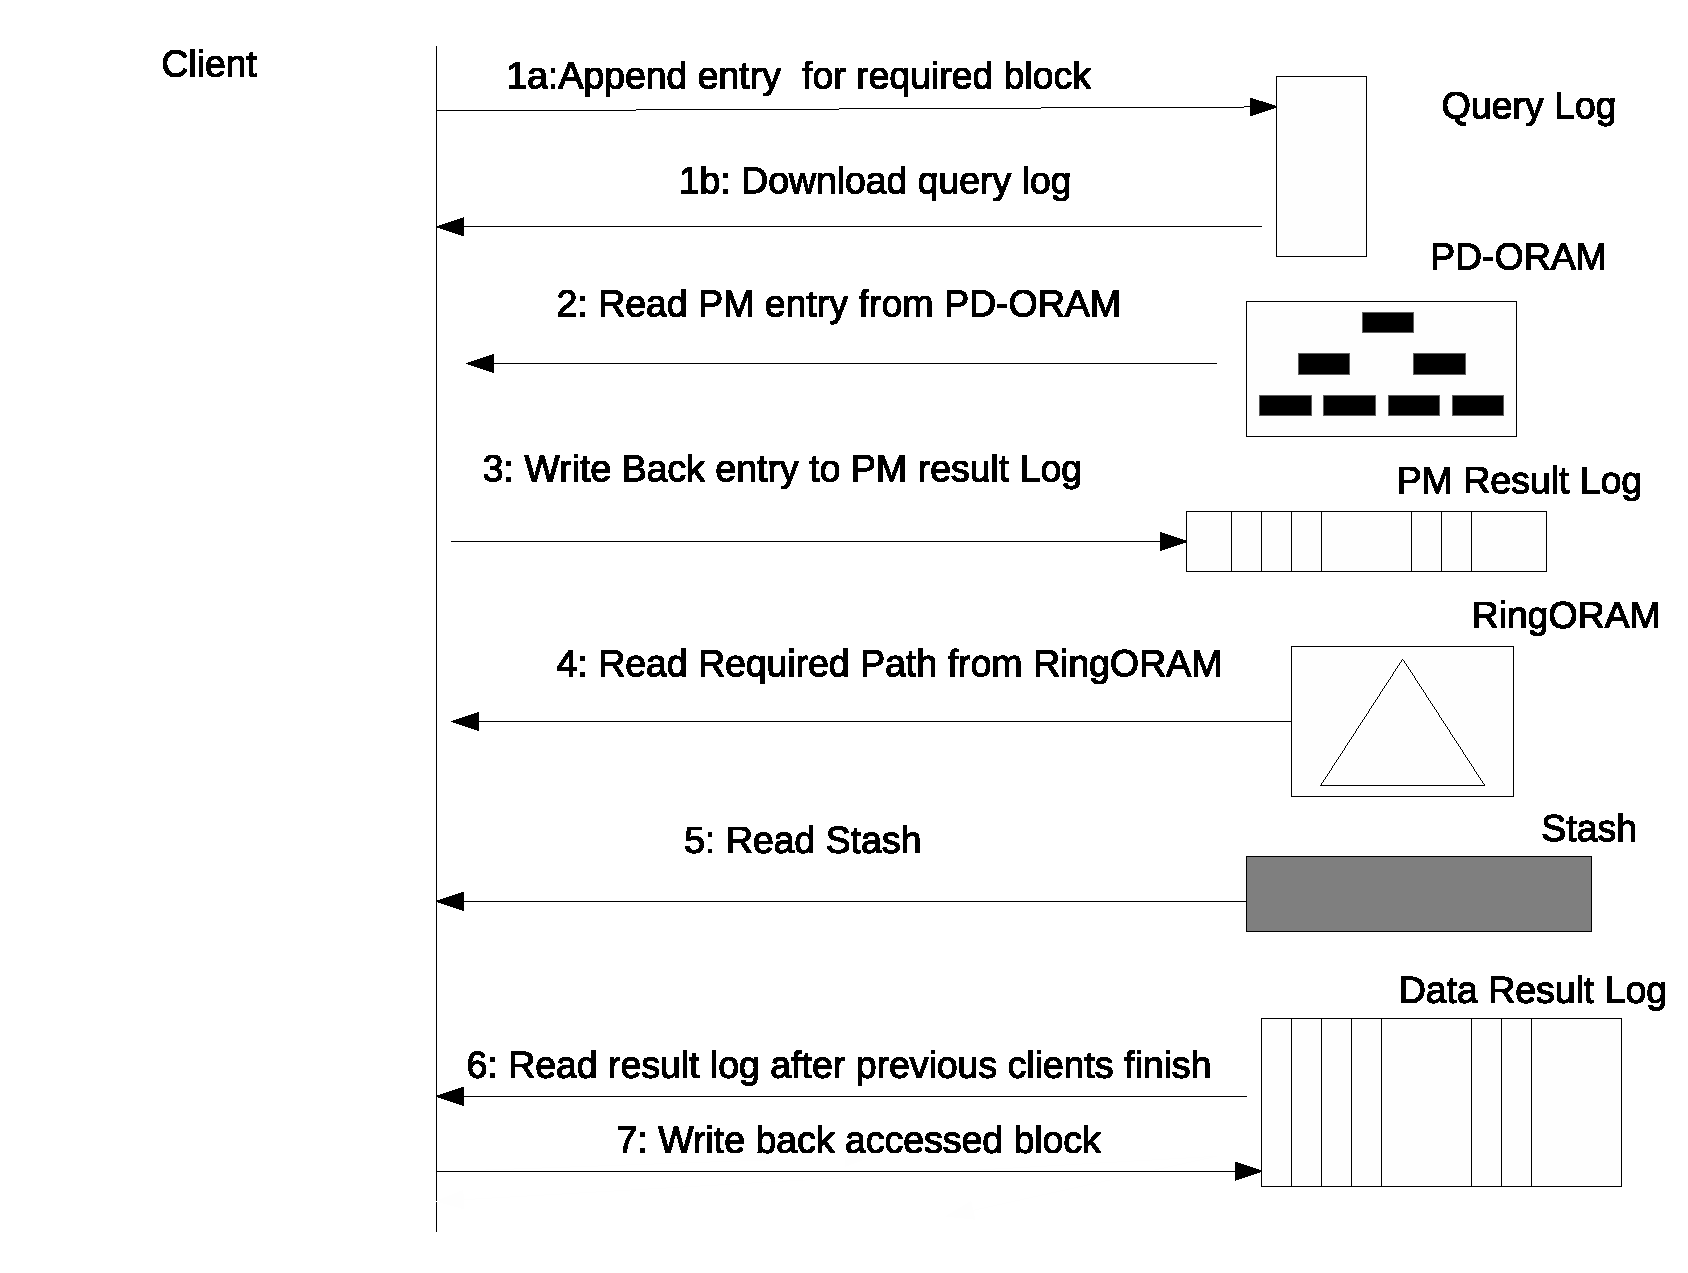
\includegraphics[scale=0.30]{Figures/Query_overview.eps}
 \caption{Overview of a query. Clients need to lock only in step 1. Steps 2-6 can proceed concurrently. In step 7, clients wait for previous clients to finish before downloading
 data result log \label{query_overview}}
\end{figure}




Figure \ref{query_overview} shows the query protocol for \sysname~. Queries proceed as follows: 
\begin{enumerate}
 \item In step 1a and step 1b, a client downloads the query log and appends the logical block ID of the block the client is querying for. If the required block 
 is already being accessed, the client appends the logical block ID of a randomly selected block and queries for the same. During step 1, the server enforces a 
 lock on the query log.
 \item In step 2, the client reads a bucket from each level of PD-ORAM to locate the position map entry for the required logical block ID. The PD-ORAM access protocol 
 ensures that the client finds the required position map entry in this step. 
 \item In step 3, the client reencrypts and writes back the actual position map entry read in Step 2 to the PM result log.
 \item In step 4 and 5, the client reads the path on which the queried block exists (as determined from the position map entry) and the stash. 
 \item In step 6, the client writes back the queried block to data result log.
 \item In step 7, the client reads the data result log after all previous clients finish. If a client has executed 
 a random query, the client gets the required block from the data result log. 
 \item If a client found the required block in step 7, the client writes back the updated value of the block to the 
 data result log for a write access. Otherwise, a client writes back a dummy block.
\end{enumerate}

Note that in step 7 a client finds the most updated version of the 
required block after all previous ongoing transactions accessing the block has completed. 




\bibliographystyle{acm}
\bibliography{Bib/references.bib}

\end{document}
